\chapter{The Experiment}\label{chap:experiment}
\minitoc
In this chapter, the relevant experimental setup is discussed. Starting with the description of the Large Hadron Collider (LHC), which is responsible for the acceleration of the proton beams, then the Compact Muon Solenoid (CMS) experiment and detector with all important subdetector components is explained.
\section{The Large Hadron Collider}\label{sec:LHC}
The Large Hadron Collider~\cite{LHC1,LHC2}, located at the European Organization of Nuclear Research (CERN) near Geneva in Switzerland, is the worlds largest hadron collider. The design center-of-mass energy for proton-proton collisions is $\sqrt{s}=14\TeV$, while the LHC started operating in 2010 with an energy of $7\TeV$. After running also in 2011 at $7\TeV$, the energy was increased for the 2012 run period to $8\TeV$. After the end of Run~I, and after the first long shutdown, the LHC started running again in 2015 with an increased center-of-mass energy of $13\TeV$. This setup was maintained trough the whole Run~II until the end of 2018. In the following, the LHC will be upgraded again in the long shutdown II, so that with the beginning of 2021 operations with the design energy of $14\TeV$ are planned.
The LHC is also capable of accelerating lead ions with an energy of $2.76\TeV$ per nucleon.\\
The LHC is a synchroton collider built in a tunnel with a circumference of $27\km$, which was already used for the Large Electron Positron collider (LEP)~\cite{LEPCollider} in the past. The proton beams are accelerated using various pre-acceleators, such as the Booster, Proton Synchroton (PS), and the Super Proton Synchroton (SPS), delivering an proton energy of $450\GeV$ before entering the main storage ring. Four main experiments are located at the LHC, each built around one of the four collisions points. These are: ALICE (A Large Ion Collider Experiment)~\cite{ALICE}, ATLAS (A Toroidal LHC Apparatus)~\cite{ATLAS}, CMS (Compact Muon Solenoid)~\cite{CMS}, and LHCb (LHC Beauty)~\cite{LHCb}. CMS and ATLAS were designed to be independent experiments, that are using different technologies, looking both now for BSM physics, measure precisely properties of the SM, and improve the knowledge of the Higgs sector. Besides those tasks, they also analyze lead ion collisions to gain a deeper understanding of the strong interaction. Initially ATLAS and CMS were designed to find the SM Higgs boson. The tasks of ALICE include studies of the quark-gluon-plasma, where the confinement is abrogated, leading to asymptotically free quarks and gluons. LHCb investigates mainly mesons that include charm and bottom quarks, to perform precision measurements of the SM and indirectly look for $\mathcal{CP}$-violation and hints for new physics. The asymmetric detector design of LHCb favors such studies, since the forward region with particles flying close to the beam axis, is enriched with that kind of events. A schematic sketch of the LHC apparatus including the four big experiment locations and interaction points, and the preaccelerators, is shown in \refFig{fig:LHC}.\\
\begin{figure}[tbp]
 \centering
 \includegraphics[width=0.89\textwidth]{figures/general/LHC}
 \caption{A sketch of the total LHC accelerator complex~\cite{LHCPicture}. The four main experiments are marked as yellow dots, and the preacceleators are also shown.}
 \label{fig:LHC}
\end{figure}
As the protons are accelerated to an energy of $450\GeV$, they are injected as bunches of approximately $N=1.1\cdot10^{10}$ particles into the two beam pipes counter rotating in intervals of $25\ns$. To achieve a center-of-mass energy of $13\TeV$, each beam has to reach an energy of $6.5\TeV$. Therefore, superconducting cavities operating at $400\MHz$ accelerate the protons, and dipole magnets force the beams on their orbital path. Higher order multipoles are needed to focus the beam and correct for different beam and magnetic effects.\\
One important quantity to characterize a collider is the instantaneous luminosity $L$, because the rate of any scattering process is proportional to $L$. It can be defined as
\begin{equation}
 % L = \frac{N_{b}^2 n_{b} f_{rev} \gamma} {4\pi \epsilon \beta^{*}}F,
 L = \frac{N_{b}^2 n_{b} f_{rev}} {4\pi \sigma{x} \sigma_{y}}F,
\end{equation}
where $N_b$ is the number of particles per bunch, $n_b$ the number of bunches, $f_{rev}$ the revolution frequency, $\sigma_{x}$ and $\sigma_{y}$ are the widths of Gaussian distributed beam profiles in x- and y-direction, and $F$ a geometrical factor accounting for the cross section angles of the beams~\cite{LuminosityConcept}. The integrated Luminosity $\Lumi_{int}$ is related to $L$ via
% where $N_b$ is the number of particles per bunch, $n_b$ the number of bunches, $f_{rev}$ the revolution frequency, $\gamma$ the relativistic Lorentz factor, $\epsilon$ the normalized transverse emmitance of the beam, $\beta^{*}$ the beta function at the interaction point, and $F$ a geometrical factor accounting for the cross section angles of the beams. The integrated Luminosity $\Lumi_{int}$ is related to $L$ via
\begin{equation}
 \Lumi_{int}= \int L dt.
\end{equation}
And the number of events $N$ for a given process with cross section $\sigma$ is given by
\begin{equation}
 N= \Lumi \cdot \sigma.
\end{equation}

In 2016 the LHC provided a total integrated luminosity of $40.82\pbinv$, while the CMS detector recorded $37.76\pbinv$, and $35.92\pbinv$ were validated as good to be used for physics analysis~\cite{DataQuality}.





% \section{The Compact Muon Solenoid detector}\label{sec:CMS}
\section{The Compact Muon Solenoid}\label{sec:CMS}
The data used in this thesis was recorded by the CMS detector~\cite{CMS,CMSTDR} in 2016. The CMS detector is a multi-purpose detector housing different subdetector components. From inside to outside these are the tracker system including a pixel and the silicon strip detector, the electromagnetic calorimeter, the hadronic calorimeter, followed by the solenoid and the muon system. A sketch of the openend CMS detector is shown in~\refFig{fig:CMS}. In the following, each subdetector and the trigger system will be briefly explained.\\
\begin{figure}[tbp]
 \centering
 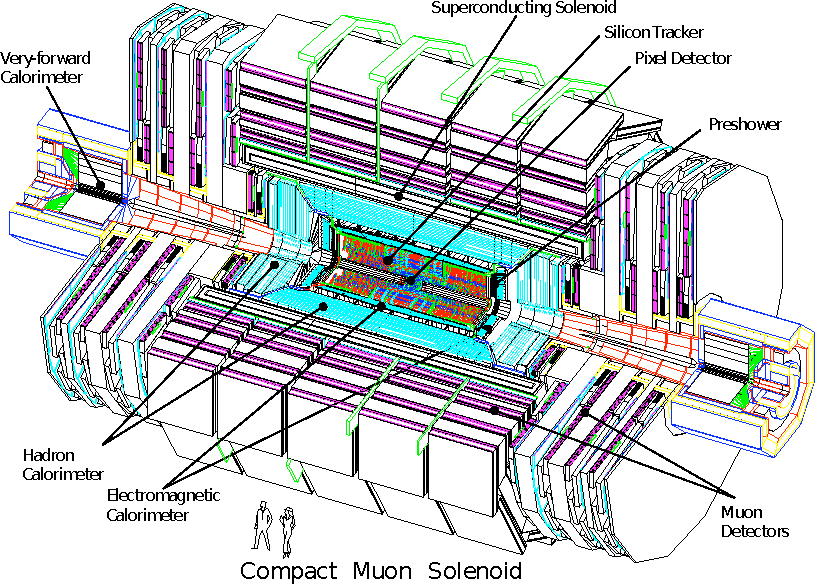
\includegraphics[width=0.99\textwidth]{figures/general/cms}
 % 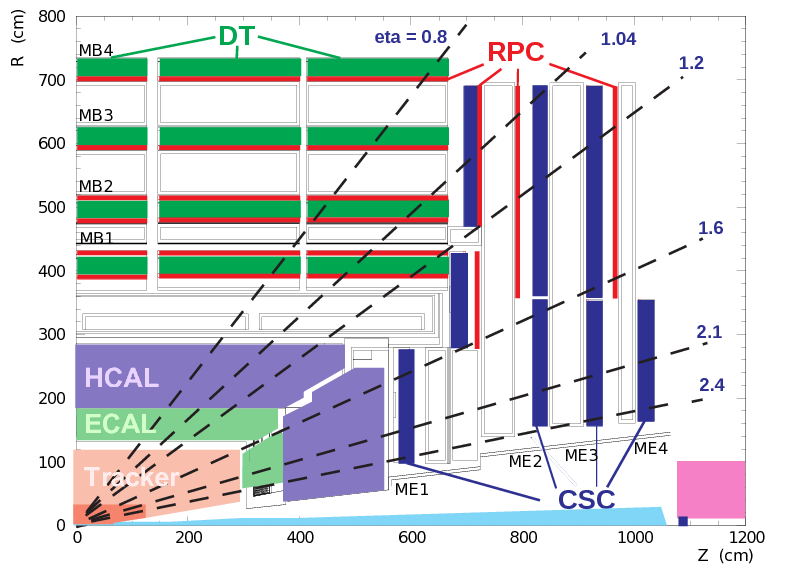
\includegraphics[width=0.49\textwidth]{figures/general/CMS_eta.png}
 \caption{A sketch of the total CMS detector with all subdetectors labeled~\cite{CMSTDR}.}
 \label{fig:CMS}
\end{figure}
The coordinate system used to describe the detector is originated at the interaction point, and the z-axis points in the direction of the beam axis toward the Jura mountains. The y-axis points upwards, while the x-axis points to the center of the LHC ring. To exploit the underlying symmetry of the detector, a transformation to an angular coordinate system is chosen. The azimuthal angle $\phi$ is measured in the x-y plane, where $\phi=0$ equals the direction of the x-axis, and $\phi$ ranges from $-\pi$ to $\pi$. The polar angle $\theta$ is measured from the positive z-axis, and the pseudorapidity $\eta$ can be introduced as
\begin{equation}
 \eta=-\ln\left(\tan\left(\frac{\theta}{2}\right)\right).
\end{equation}
The advantage in using $\eta$ instead of $\theta$ is, that differences in $\eta$ are invariant under Lorentz-boosts along the beam axis, and in the high energy limit the pseudorapidity equals the rapidity.\\
In proton proton collisions, the initial total momentum of the colliding partons is unknown, since they carry only a fraction of the proton energy. But, the transverse momentum in the initial state is negligible, and therefore, the transverse momentum
\begin{equation}
 \pt=|\ptvec|=|\vec{p}\cdot\sin(\theta)|
\end{equation}
is a widely used quantity.
Most of the subdetectors are divided in a low $\eta$ part (barrel), and two high $\eta$ parts (endcaps). Each of the subdetectors is designed to measure special properties of different particle types, to ensure both a good particle distinction and identification, and precise measurements of energy, momenta, and trajectories.



\subsection{Tracker system}
The most inner part of the CMS detector is the inner tracker, and it consists of two main components, a silicon pixel and a silicon strip detector\footnote{The silicon pixel detector was replaced at the end of the 2016 run. Since in this thesis only 2016 data is used, only the former detector is discussed.}. Both components enclose parts parallel to the beam pipe in the barrel, and parts orthogonal to the beam axis in the endcaps. They cover a length of $5.8\m$ and a diameter of $2.5\m$. A sketch of the total inner tracker divided in all subparts is shown in \refFig{fig:tracker}. The tracker is designed to perform a precise measurement of particle trajectories and an identification of primary and secondary vertices. Therefore, a high granularity and fast response is needed. The silicon pixel subcomponent is built of three barrel layers (the closest at a radial distance of $4.4\cm$ to the center of the beam pipe) and two endcap disks, covering a total area size of around $1\m^2$. Each of the $\approx66$ million silicon pixel cells has a size of $100\times150\micron^2$. This enables good resolution in all orientations independent of the track direction.\\
The silicon strip detector consists of four strip layers in the inner (TIB), and six layers in the outer part (TOB). In the direction of the endcaps, it is built of three inner disk layers (TID), and nine layers in the outer part (TEC).\\
The inner tracker in total covers a range of $|\eta|<2.5$ and the total sensoring system has a size of around $200\m^2$. The performance of the tracker yields a momentum resolution for muons with a transverse momentum of $\approx100\GeV$ of $1-2\%$ in the pseudorapidity range of $|\eta|<1.6$. At higher pseudorapidities the momentum resolution decreases due to a lower granularity.

\begin{figure}[tbp]
 \centering
 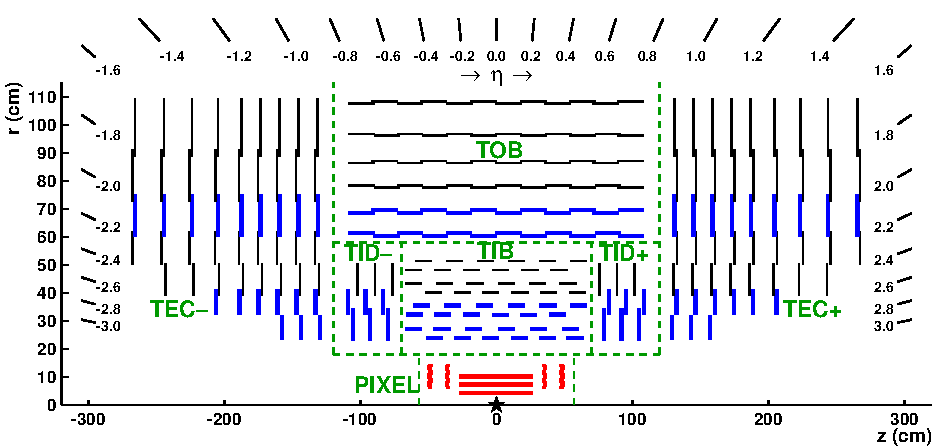
\includegraphics[width=0.79\textwidth]{figures/general/tracker.pdf}
 \caption{A sketch of one quadrant of the CMS inner tracker~\cite{TrackerPDFPic}.}
 \label{fig:tracker}
\end{figure}

\subsection{Electromagnetic calorimeter}
Around the tracker, the second subdetector of CMS is the electromagnetic calorimeter (ECAL). Its main purpose is to measure the energy of electrons and photons, which behave very similar in the calorimeter. Only with the combined measurements of the tracker, a differentiation between electrons and photons can be performed. It is made homogeneously of lead-tungstate ($PbWO_4$) crystals, that emit light proportional to the deposited energy of traversing particles in an electromagnetic shower. The emitted light in the visible spectrum is measured by avalanche photomultipliers. The material of lead-tungstate was chosen due to its high density, short Moli\`{e}re radius of $2.2\cm$ characterizing the shower width, and short radiation length of $0.89\cm$. Another big advantage of $PbWO_4$ is the short scintillation time. In a time window of $25\ns$ most of the visible light ($\approx80\%$) is emitted, thus suiting very well the bunch spacing of $25\ns$. The ECAL is divided into a barrel (EB: $|\eta|<1.479$) and an endcap part (EE: $1.479<|\eta|<3.0$), as can be seen in \refFig{fig:etaPlaneCMS}. The $61200$ crystals mounted in the barrel have a length of $23\cm$, resulting in $25.8$ radiation lengths, and cross section of $22\times22\mm^2$ matching the Moli\`{e}re radius of $PbWO_4$. In each ECAL endcalp, $3662$ crystals are placed, having a larger cross section of $ 28.6\times28.6\mm^2$ and a length of $22\cm$.
To prevent particle trajectories to align with the orientation of ECAL crystal borders, the crystals (in EB) are tilted in an angle of $3$ degree with respest to their otientation toward the interaction point. In the EE, the tilting varies between $2-8$ degree in dependence of $\eta$. So in total both a compact format and a high granularity could be maintained.\\
\begin{figure}[tbp]
 \centering
 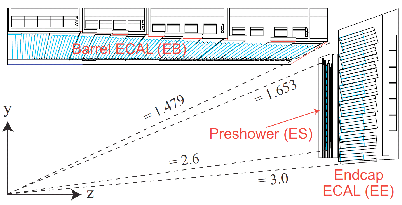
\includegraphics[width=0.49\textwidth]{figures/general/ecal}
 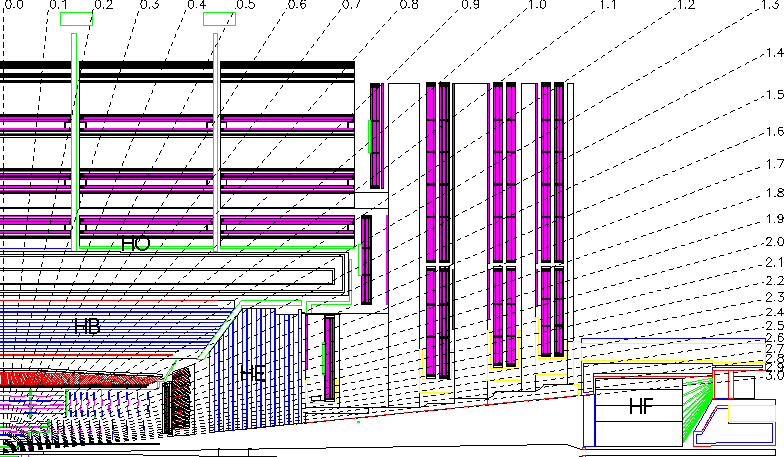
\includegraphics[width=0.49\textwidth]{figures/general/hcal}
 \caption{A sketch of one quadrant of the CMS detector for the ECAL (left)~\cite{ECALPicture}, and HCAL (right)~\cite{CMS}.}
 \label{fig:etaPlaneCMS}
\end{figure}
The total energy resolution of the ECAL is determined to be
\begin{equation}
 \left(\frac{\sigma_E}{E}\right)^2=\left(\frac{2.8\%}{\sqrt{E[\GeV]}}\right)^2 + \left(\frac{0.12}{E[GeV]}\right)^2 + (0.30\%)^2,
\end{equation}
where the first term covers stochastic effects due to the Poissonian distributed number of created scintillation photons, and the second term combines noise effects both from the electronics and multiple collisions per bunch-crossing (pileup). The third term covers constant effects, such as intercalibration effects between the crystals and energy leakage. All the values were obtained in a teast beam setup~\cite{ECALRes}. The energy resolution was designed to be optimal at eneries of around $\approx50\GeV$ to maximise the sensitivity for the Higgs boson discovery, where photons from the photonic Higss decay were expected.\\
An additional preshower detector is installed in front of the ECAL endcap, to identify photons coming from meson decays.

\subsection{Hadronic calorimeter}
The hadronic calorimeter (HCAL), which is designed for the energy measurement of hadrons, consists also of a barrel (HB) and endcap parts (HE). It is placed between the ECAL at a radius of $1.77\m$ and the magnet coil at a radius of $2.95\m$. An additional outer barrel part with lower granularity (HO) extends the HCAL outside of the solenoid, making use of its stopping power, while the hadron forward (HF) is installed to cover high pseudorapidity ranges. The barrel part covers pseudorapidities in the range of $|\eta|<1.4$, while the HCAL endcap together with the outer HCAL covers the range of $1.3<|\eta|<3$.\\
In contrast to the homogeneous ECAL, the HCAL barrel is a so called sampling calorimeter, consisting of alternating layers of brass and plastic scintillating material. The front and backplates are made of steel. Hence, the brass plates stop the incoming particles, and the energy deposit is measured in the form of hadronic showers creating scintillation light in the plastic layers. The outer HCAL makes use of the same principle, but uses in addition the stopping power of the solenoid. The hadron forward, covering pseudorapidity ranges of $3<|\eta|<5.2$, needs to be more radiation hard in comparison to the rest of the HCAL, since the energy deposit in the forward region is much higher. It is therefore constructed as a Cherenkov detector made of quartz fibres. A total sketch of the HCAL can be seen in \refFig{fig:etaPlaneCMS}.

\subsection{The solenoid}
To measure the momentum of the  charged particles properly, it is crucial to have bended trajectories. The resolution of the momentum measurement at very high energies is directly proportional to the particles momentum. Thus, for a precise measurement of the curvature of the trajectory, a strong magnetic field is needed. In case of the CMS detector, this is provided by a superconducting NbTi magnet, cooled down to $4.8\K$, inducing a magnetic field of $3.8\T$. By choosing a solenoid with a length of $12.5\m$ and a diameter of $6.3\m$, the solenoid defines the CMS detector design.
% \todo{Erganzen!}

\begin{figure}[tbp]
 \centering
 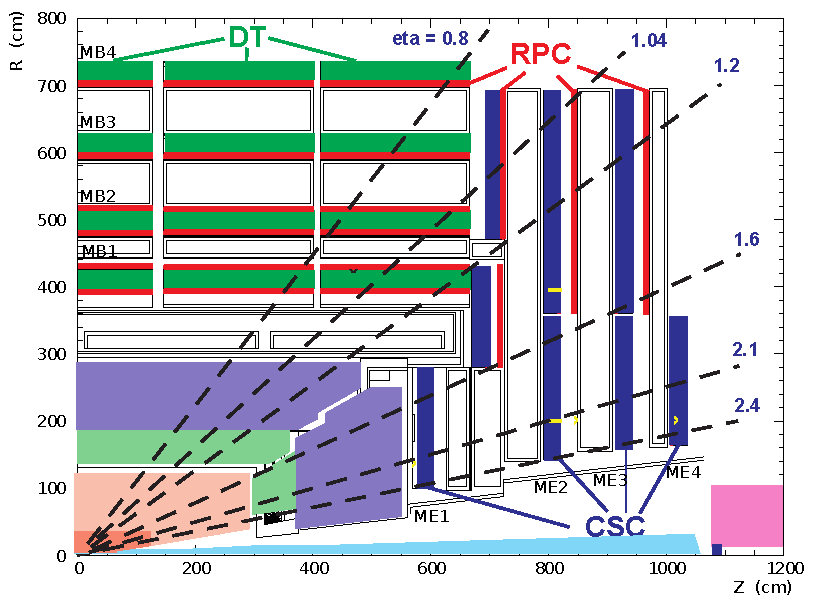
\includegraphics[width=0.65\textwidth]{figures/general/muonChamber}
 \caption{A sketch of one quadrant of the CMS detector is shown with the main detector components~\cite{CMSTDR}.}
 \label{fig:etaPlaneCMSTotal}
\end{figure}

\subsection{Muon system}
The most outside part of the CMS detector is the muon system. Because all other particles besides muons should be stopped in the inner layers, muons are the only particles entering the muon system and leaving a signature there. Three different types of detectors are used to measure and identify muons. The barrel part ($|\eta|<1.2$) is covered by four stations of drift tubes (DT). Cathode strip chambers (CSC) are covering the endcap at pseudorapidity $0.9<|\eta|<2.4$, because in this region a higher muon rate is expected, and CSCs in contrast to DTs have a faster response time and are more radiation hard. In most of the parts the reconstructed muon efficiency is above $95\%$, with a misidentification of less than $1\%$. The muon momentum resolution, dependent on the $\eta$ region, varies between $1\%$ to $6\%$ for muons with a transverse momentum below $100\GeV$, and is of the order of $10\%$ for $\TeV$ muons~\cite{MuonPerformance}. Again, the energy resolution was designed to be at its maximum at $\approx50\GeV$, where muons from the diboson Z decays of the Higgs boson were expected.\\
Additional detector components, namely six layers of resistive plate chambers (RPC), are installed in the pseudorapidity range of $|\eta|<1.8$. Because they show both good time resolution and fast response time, they are mainly used for triggering purposes. The structure of the muon system can be seen in \refFig{fig:etaPlaneCMSTotal}.

\subsection{Trigger system}
As collisions take place every $25\ns$, and therefore at a rate of $40\MHz$, it is not achievable to read out and store all events. To keep only physically interesting events and reduce the rate of events to be saved, a trigger system consisting of two stages is implemented~\cite{TriggerSystem}. It is composed of the hardware based level 1 triggers (L1), and the software based high level triggers (HLT). Since the L1 trigger needs to deliver decisions in a very short time window, it uses only information provided by the calorimeters and the muon chambers. Usually first requirements on the event, such as a minimal deposited transverse energy, and  the presence of first estimates for electron and muon candidates, are imposed. The L1 trigger reduces the event rate to a rate of $\approx100\kHz$.\\
A more complex decision taking is done by the HLT trigger system. It has full access to the total readout of all subdetectors, and therefore performs selections close to the offline analysis. It reduces the event rate to $\mathcal{O}(1\kHz)$~\cite{TriggerRate}.\\
Using the decisions of the HLT, events are categorized into different subsets, based on event kinematics and the trigger objects.
